\documentclass[border=6pt]{standalone}
\usepackage{tikz}
\usetikzlibrary{arrows.meta}
\begin{document}
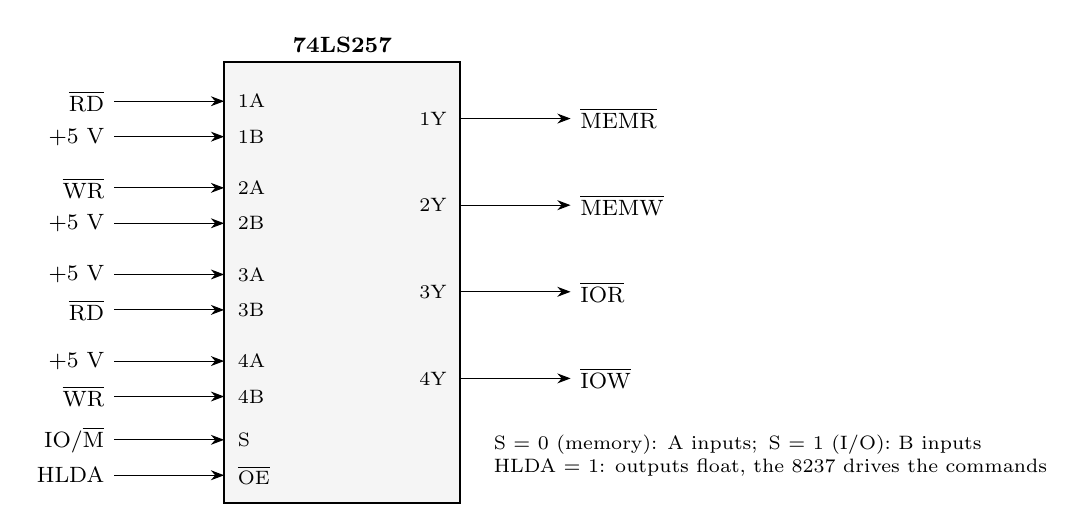
\begin{tikzpicture}[>=Stealth,font=\small]
\draw[thick,fill=gray!8] (0,0) rectangle (3.0,-5.6);
\node[font=\footnotesize\bfseries,anchor=south] at (1.5,0) {74LS257};
\foreach \k/\y/\a/\b/\o in {1/-0.5/$\overline{\mathrm{RD}}$/+5 V/$\overline{\mathrm{MEMR}}$,2/-1.6/$\overline{\mathrm{WR}}$/+5 V/$\overline{\mathrm{MEMW}}$,3/-2.7/+5 V/$\overline{\mathrm{RD}}$/$\overline{\mathrm{IOR}}$,4/-3.8/+5 V/$\overline{\mathrm{WR}}$/$\overline{\mathrm{IOW}}$} {
  \node[font=\scriptsize,anchor=west] at (0.05,\y) {\k A};
  \node[font=\scriptsize,anchor=west] at (0.05,\y-0.45) {\k B};
  \node[font=\scriptsize,anchor=east] at (2.95,\y-0.22) {\k Y};
  \draw[<-] (0,\y) -- (-1.4,\y) node[left,font=\footnotesize]{\a};
  \draw[<-] (0,\y-0.45) -- (-1.4,\y-0.45) node[left,font=\footnotesize]{\b};
  \draw[->] (3.0,\y-0.22) -- (4.4,\y-0.22) node[right,font=\footnotesize]{\o};
}
\node[font=\scriptsize,anchor=west] at (0.05,-4.8) {S};
\node[font=\scriptsize,anchor=west] at (0.05,-5.25) {$\overline{\mathrm{OE}}$};
\draw[<-] (0,-4.8) -- (-1.4,-4.8) node[left,font=\footnotesize]{IO/$\overline{\mathrm{M}}$};
\draw[<-] (0,-5.25) -- (-1.4,-5.25) node[left,font=\footnotesize]{HLDA};
\node[font=\scriptsize,align=left,anchor=west] at (3.3,-5.0) {S = 0 (memory): A inputs;\enspace S = 1 (I/O): B inputs\\HLDA = 1: outputs float, the 8237 drives the commands};
\end{tikzpicture}
\end{document}
